\documentclass[11pt,a4paper]{article}
\pdfoutput=1
\usepackage{jheppub}
\usepackage{latexsym,amsmath,amssymb}
\usepackage{graphicx}
\DeclareGraphicsRule{*}{mps}{*}{}
\usepackage[table,usenames,dvipsnames]{xcolor}
\usepackage{hyperref}
\definecolor{azure(colorwheel)}{rgb}{0.0, 0.5, 1.0}
\hypersetup{colorlinks=true,linkcolor=blue,citecolor=azure(colorwheel),pdfborder={0 0 0}}
\usepackage[utf8]{inputenc}
\usepackage{feynmp}
\usepackage{lipsum}
\newcolumntype{P}[1]{>{\centering\arraybackslash}p{#1}}


\newcommand{\Tr}{\mathrm{Tr}} 
\newcommand{\STr}{\mathrm{STr}}
\newcommand{\D}{\mathrm{d}}
\newcommand{\vev}[1]{\langle #1 \rangle}
\newcommand{\spinup}{\uparrow}
\newcommand{\spindown}{\downarrow}
\newcommand{\marrow}[5]{%
    \fmfcmd{style_def marrow#1
    expr p = drawarrow subpath (1/4, 3/4) of p shifted 6 #2 withpen pencircle scaled 0.4;
    label.#3(btex #4 etex, point 0.5 of p shifted 6 #2);
    enddef;}
    \fmf{marrow#1,tension=0}{#5}}
\newcommand*\DAlambert{\mathop{}\!\mathbin\Box}

\makeatletter
\newcommand*{\rom}[1]{\expandafter\@slowromancap\romannumeral #1@}
\makeatother

% highlights
\newcommand{\draftnote}[1]{\textbf{#1}}
\newcommand{\fixme}[1]{{\bf {\color{red}[#1]}}}% comments, questions
\newcommand{\ignore}[1]{}
\newcommand{\RED}[1]{{\color{red} #1}}
\newcommand{\todo}[1]{{\color{ForestGreen} [TO DO: #1]}}% things to-do/to write
\newcommand{\tent}[1]{{\color{blue} #1}}% tentative sentences
\newcommand{\hl}{\color[rgb]{0,0.4,0.6}}
\newcommand{\alert}{\color[rgb]{1,0,0}}
% \newcommand{\okay}{\color{ForestGreen}}
\newcommand{\okay}[1]{[#1]}
\newcommand{\IBM}[1]{{\color{cyan} [IBM: #1]}}% things to-do/to write
\newcommand{\CS}[1]{{\color{magenta} [CS: #1]}}% things to-do/to write
\newcommand{\TV}[1]{{\color{red} [TV: #1]}}% things to-do/to write
\newcommand{\NO}[1]{{\color{blue} [NO: #1]}}% things to-do/to write
\newcommand{\DR}[1]{{\color{purple} [DR: #1]}}% things to-do/to write


%
%
%
%
%
%
\notoc
\begin{document}%in the revtex template, the title and author info should be included after the begin doc command.
\title{
  A Demonstration of past.el
}

\author[a]{Chen Sun,}
\affiliation[a]{School of Physics and Astronomy, Tel-Aviv University, Tel-Aviv 69978, Israel}
\emailAdd{chensun@mail.tau.ac.il}

% \abstract{
% This is a unfinished note to study the measurement of $f_{\rm gas}$ and using it to constrain cosmological and axion parameters.
% }

\date{\today}

% \begin{abstract}
% We have a paper that rocks!
% \end{abstract}

% \pacs{xxx.xxx}   

% \preprint{xxx-xxx}

\maketitle

%\tableofcontents

\lipsum[20]

\begin{figure}[ht]
    \centering
    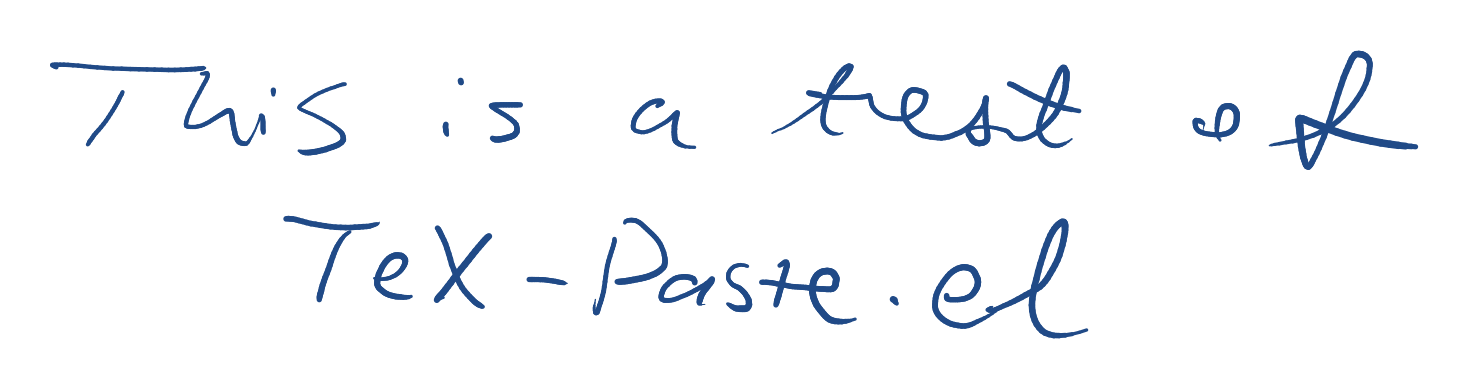
\includegraphics[width=.8\textwidth]{drawings/testfigure.png}
    \label{fig:testfigure}
    \caption{}
\end{figure}

\lipsum[20]


%\nocite{*}
\bibliography{bib}
\bibliographystyle{utphys}
\end{document}





















%%% Local Variables:
%%% mode: latex
%%% TeX-master: t
%%% End:




